\documentclass[11pt,a4paper]{article}

\usepackage[T1]{fontenc}
\usepackage[utf8]{inputenc}
\usepackage{mathptmx}
\usepackage[margin=2.4cm]{geometry}
\usepackage{amsmath}
\usepackage{booktabs}
\usepackage{graphicx}
\usepackage{microtype}
\usepackage[font=small,labelfont=bf]{caption}
\usepackage{siunitx}
\usepackage{xcolor}
\usepackage[colorlinks=true,allcolors=blue!55!black]{hyperref}
\usepackage{titlesec}
\titleformat{\section}{\normalfont\large\bfseries}{\thesection}{0.6em}{}
\titleformat{\subsection}{\normalfont\normalsize\bfseries}{\thesubsection}{0.6em}{}
\setlength{\parskip}{0.35em}
\setlength{\parindent}{0pt}

% generated by examples/make_report_numbers.py -- do not edit
\newcommand{\selNrep}{400}
\newcommand{\selNcond}{112}
\newcommand{\selNprof}{44\,800}
\newcommand{\RecRtwo}{37\%}
\newcommand{\RecAdj}{68\%}
\newcommand{\RecAICc}{77\%}
\newcommand{\RecBIC}{73\%}
\newcommand{\Disagree}{67\%}
\newcommand{\MeanBestRtwo}{0.9893}
\newcommand{\GapMedian}{0.00072}
\newcommand{\GapNinety}{0.0046}
\newcommand{\NparRtwo}{1.86}
\newcommand{\NparAICc}{1.19}
\newcommand{\RecRtwoOnePar}{17.7\%}
\newcommand{\RecAICcOnePar}{89\%}
\newcommand{\RecRtwoTwoPar}{84\%}
\newcommand{\RecAICcTwoPar}{46\%}
\newcommand{\NOnePar}{32\,000}
\newcommand{\HigPickRtwo}{Korsmeyer-Peppas}
\newcommand{\HigPickRtwoF}{94\%}
\newcommand{\HigPickAICcF}{89\%}
\newcommand{\FoPickRtwo}{Weibull}
\newcommand{\FoPickRtwoF}{96\%}
\newcommand{\KPPickAICc}{Baker-Lonsdale}
\newcommand{\KPPickAICcF}{62\%}
\newcommand{\KPRecAICc}{31\%}
\newcommand{\KPRecRtwo}{80\%}
\newcommand{\RecAICcLowNoise}{92\%}
\newcommand{\RecAICcHighNoise}{60\%}
\newcommand{\RecAICcSix}{71\%}
\newcommand{\RecAICcSixteen}{81\%}
\newcommand{\mechNrep}{150}
\newcommand{\mechNboot}{200}
\newcommand{\mechNcond}{60}
\newcommand{\mechKept}{6.7}
\newcommand{\mechKeptMin}{4.0}
\newcommand{\BiasNLS}{-0.004}
\newcommand{\BiasLog}{+0.011}
\newcommand{\RmseNLS}{0.063}
\newcommand{\RmseLog}{0.116}
\newcommand{\Coverage}{79.8\%}
\newcommand{\CIWidth}{0.17}
\newcommand{\SingleClass}{47\%}
\newcommand{\ClassCorrectNLS}{82\%}
\newcommand{\ClassCorrectLog}{77\%}
\newcommand{\MethodsAgree}{85\%}
\newcommand{\SingleClassBest}{69\%}
\newcommand{\SingleClassWorst}{28\%}
\newcommand{\CIWidthBest}{0.06}
\newcommand{\CIWidthWorst}{0.33}
\newcommand{\BestGrid}{12}
\newcommand{\WorstGrid}{6}
\newcommand{\SigLo}{1}
\newcommand{\SigHi}{5}
\newcommand{\RmseRatio}{1.8}
\newcommand{\ClassCorrectInterior}{97\%}
\newcommand{\ClassCorrectBoundary}{61\%}
\newcommand{\SingleClassInterior}{68\%}
\newcommand{\SingleClassBoundary}{17\%}
\newcommand{\InteriorNs}{0.35, 0.60, 0.75}
\newcommand{\BoundaryNs}{0.45, 0.95}
\newcommand{\CovSix}{73\%}
\newcommand{\KeptSix}{4.6}
\newcommand{\CovEight}{80\%}
\newcommand{\KeptEight}{6.2}
\newcommand{\CovTwelve}{87\%}
\newcommand{\KeptTwelve}{9.4}
\newcommand{\Disagreeance}{15\%}
\newcommand{\DisagreeOneIn}{7}
\newcommand{\calNrep}{200}
\newcommand{\calNboot}{250}
\newcommand{\calNtrue}{0.60}
\newcommand{\calSigma}{2}
\newcommand{\CovPlain}{80.5\%}
\newcommand{\CovResc}{88.3\%}
\newcommand{\RatioPlain}{0.76}
\newcommand{\RatioResc}{0.96}
\newcommand{\CovPlainSix}{71.5\%}
\newcommand{\CovRescSix}{87.0\%}
\newcommand{\CovPlainTwelve}{90.5\%}
\newcommand{\CovRescTwelve}{92.0\%}
\newcommand{\fNmc}{2\,000}
\newcommand{\fFarAcc}{99.4\%}
\newcommand{\fFarWorst}{90.9\%}
\newcommand{\fNearAcc}{47\%}
\newcommand{\fIdentBias}{-12.2}
\newcommand{\fIdentWorst}{75}
\newcommand{\fIdentWorstSD}{6}
\newcommand{\fIdentWorstN}{6}
\newcommand{\fBiasNonIdent}{+0.11}
\newcommand{\fWorked}{50.2}
\newcommand{\fWorkedLo}{47.7}
\newcommand{\fWorkedHi}{52.4}
\newcommand{\fWorkedP}{49\%}
\newcommand{\fSDsmall}{0.59}


\title{\bfseries How often does $R^2$ pick the right release model?\\[0.25em]
\large A simulation study of model selection and mechanism assignment\\
in dissolution kinetics}
\author{Kancharla Nithya Sri\\[0.2em]
\small M.\,Pharm (Pharmaceutics)\\
\small \texttt{dissokin}: an open source Python toolkit and reproducible study}
\date{September 2026}

\begin{document}
\maketitle

\begin{abstract}
\noindent
Release kinetics from an in vitro dissolution profile are routinely assigned
by fitting a panel of models and reporting the one with the highest $R^2$, and
the transport mechanism is then read off the Korsmeyer-Peppas exponent $n$
as a point estimate with no interval. This report tests both practices
against known ground truth. \selNprof{} profiles were simulated from seven
release laws across four sampling schedules and four assay noise levels, and
all eight candidate models were fitted to each. Selecting by $R^2$ recovered
the generating model in \RecRtwo{} of profiles; selecting by AICc recovered it
in \RecAICc{}. The two rules disagreed on \Disagree{} of profiles. The failure
is systematic rather than noisy: where the truth had one free parameter, $R^2$
recovered it in \RecRtwoOnePar{} of \NOnePar{} profiles, because a richer
model can only fit at least as well and $R^2$ charges nothing for the extra
parameter. On data generated by pure Higuchi
diffusion, $R^2$ named Korsmeyer-Peppas in \HigPickRtwoF{} of cases, which is
the single most common conclusion in the applied literature. A second
experiment estimated $n$ under the conventional 60\,\% truncation rule, which
left \KeptSix{} usable points on a six point schedule. Whether a mechanism can
be assigned turned almost entirely on distance from a Ritger-Peppas boundary:
for true exponents at least $0.10$ from one the classification was correct in
\ClassCorrectInterior{} of profiles, and for exponents within $0.06$ of one in
\ClassCorrectBoundary{}, which the point estimate gives no way to tell apart.
The log-log linearisation used in most published analyses carried
\RmseRatio{} times the root mean square error of nonlinear least squares, and
the two conventions assigned different mechanisms to the same profile in
\Disagreeance{} of cases. The $f_2$ similarity factor, by contrast, proved
well behaved: away from the threshold its decision was correct in \fFarAcc{}
of studies. A calibration experiment turned the same scepticism on the method used
here and found the residual bootstrap itself undercovers at these sample
sizes, \CovPlain{} against a nominal 95\,\%, with rescaling of the residuals
by $\sqrt{n/(n-k)}$ recovering \CovResc{}. The
accompanying package implements information-criterion ranking with Akaike
weights and bootstrap intervals as defaults.
\end{abstract}

\section{The practice being tested}

An in vitro release profile is a small dataset. A dissolution monograph
typically specifies six to twelve sampling points, and the assay behind each
one carries a standard deviation of a few percent released. Against that
dataset it is standard to fit the classical release models
\cite{higuchi1963,korsmeyer1983,costa2001}, tabulate $R^2$ for each, declare
the largest the ``best fit model'', and, if Korsmeyer-Peppas is the winner,
quote its exponent $n$ and assign a transport mechanism from the
Ritger-Peppas boundaries \cite{ritger1987a,ritger1987b}. The most widely used
tool for this, DDSolver \cite{zhang2010}, reports $R^2$, adjusted $R^2$, AIC
and the model selection criterion side by side, so the choice of rule is left
to the analyst, and $R^2$ is the one that reaches the paper.

Two things are wrong with this in principle. First, $R^2$ never decreases when
a parameter is added, so comparing a one-parameter model against a
two-parameter model on $R^2$ is not a comparison at all; the richer model wins
whenever the models are nested and is heavily favoured when they are not.
Second, $n$ is an estimate from a handful of points and carries sampling
error, but the mechanistic boundaries it is compared against
($0.45$ and $0.89$ for a slab) are treated as though it did not.

Neither objection is new; both are ordinary statistics. What is not
established is how much they matter at the sample sizes and noise levels
dissolution work actually operates at. A textbook can say that $R^2$ favours
the richer model without telling you whether that changes the conclusion once
in fifty profiles or once in three. Answering it needs the true generating
model, which no real dataset provides, so the only route is simulation. That
is what the rest of this report does.

\section{Methods}

\subsection{Models}

Eight release laws are implemented, each mapping time $t$ in hours to
cumulative percent released $Q$: zero order ($Q=k_0t$), first order
($Q=100[1-e^{-k_1t}]$), Higuchi \cite{higuchi1961,higuchi1963}
($Q=k_H\sqrt{t}$), Korsmeyer-Peppas \cite{korsmeyer1983}
($Q=k_{KP}t^{\,n}$), Hixson-Crowell \cite{hixson1931}
($Q=100[1-(1-k_{HC}t)^3]$), Weibull \cite{langenbucher1972}
($Q=100[1-e^{-t^{\beta}/\alpha}]$), Hopfenberg \cite{hopfenberg1976}
($Q=100[1-(1-k_{HB}t)^{n}]$) and Baker-Lonsdale \cite{baker1974}, which is
implicit,
\begin{equation}
\tfrac{3}{2}\left[1-\left(1-\tfrac{Q}{100}\right)^{2/3}\right]-\tfrac{Q}{100}
= k_{BL}\,t ,
\end{equation}
and is inverted here by a vectorised bisection on $Q$ rather than by the usual
linearisation, so that the fit is performed in the same units as the data.

Hopfenberg reduces exactly to Hixson-Crowell at $n=3$. In the original
formulation $n$ is fixed by device geometry and is not estimated; fitting it
freely, as is common, makes the model degenerate, and on data that
Hixson-Crowell describes well the optimiser drives $n$ to the bound and the
two return identical residual sums of squares. Both are retained here because
both appear in the literature. Ties in $R^2$ are broken in favour of the
model listed first, which is the simpler one. That convention is generous to
$R^2$, so it makes the conclusions below conservative rather than the reverse.

\subsection{Selection criteria}

For least squares with unknown constant variance, the maximised log likelihood
gives AIC \cite{akaike1974} and its small sample correction
\cite{hurvich1989} as
\begin{equation}
\mathrm{AIC} = n\ln\!\left(\frac{\mathrm{RSS}}{n}\right) + 2(k+1),
\qquad
\mathrm{AICc} = \mathrm{AIC} + \frac{2(k+1)(k+2)}{n-k-2},
\end{equation}
where $k$ counts the model parameters and the $+1$ counts the variance. The
small-sample correction is not optional here: at $n=6$ and $k=2$ the
correction term is larger than the penalty it corrects. BIC \cite{schwarz1978} is reported alongside for comparison. Akaike weights
$w_i \propto \exp(-\tfrac{1}{2}\Delta_i)$ \cite{burnham2002} accompany the
ranking, because a profile that cannot distinguish two models should say so
rather than name a winner.

\subsection{Simulation}

Profiles were generated from a known model and parameters, evaluated on a
sampling schedule, and perturbed by additive Gaussian noise of standard
deviation $\sigma$ in percent released, then clipped to $[0,100]$ because an
assay cannot report a negative or above-label release. Parameters were chosen
so that each scenario reaches 75 to 96\,\% released over a twelve hour window,
which is the regime in which the models are genuinely hard to separate.
Schedules were geometric in time, matching the dense-early pattern of a real
monograph, at 6, 8, 10 and 16 points; $\sigma \in \{1,2,3,5\}$. Every draw is
seeded, so all numbers in this report regenerate exactly.

\subsection{The 60 percent rule}

The Korsmeyer-Peppas power law is derived for the early stage of release and
is conventionally fitted only below about 60\,\% released
\cite{ritger1987a,peppas1985}. Experiment 2
applies the rule honestly, keeping the leading run of points below the cutoff.
This is not a technicality: it is what leaves a two-parameter model with a
median of \mechKept{} points, and in the sparsest condition \mechKeptMin{}.

\section{Experiment 1: which selection rule recovers the truth?}

\subsection{One profile, eight answers}

Figure~\ref{fig:ident} makes the problem concrete on a single profile
simulated from Higuchi diffusion at $\sigma=2$. Korsmeyer-Peppas attains
$R^2=0.99327$ against Higuchi's $0.99320$. On the usual rule Higuchi loses,
and the report would state that release follows Korsmeyer-Peppas with
$n=0.49$, indicating anomalous transport. In fact $n=0.49$ is Higuchi
($n=\tfrac{1}{2}$) with an extra parameter spent, the margin is $7\times
10^{-5}$ in $R^2$, and AICc places $94\,\%$ of its weight on Higuchi.

\begin{figure}[t]
\centering
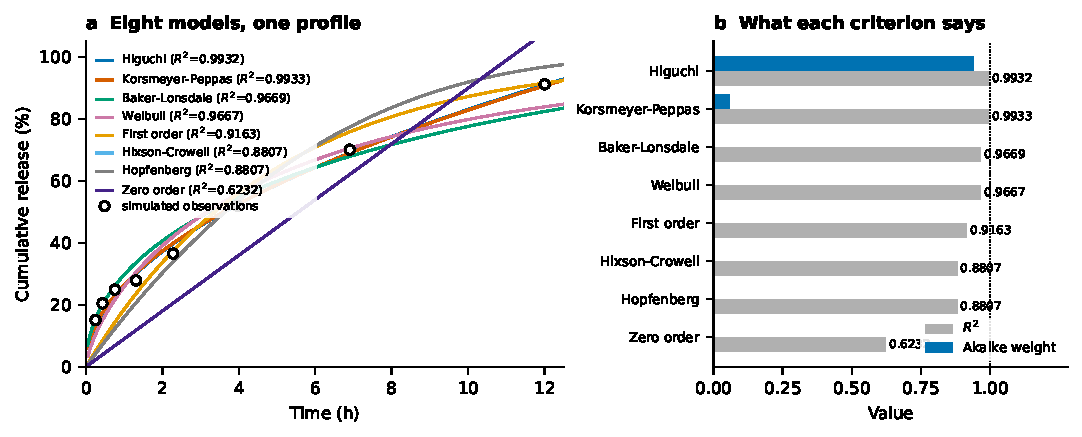
\includegraphics[width=\textwidth]{../figures/fig1_identifiability.pdf}
\caption{\textbf{Eight release models are nearly indistinguishable on one
profile.} Data simulated from Higuchi diffusion, eight points,
$\sigma=2\,\%$. (a) All eight fitted curves. (b) $R^2$ separates the leading
models in the fourth decimal; the Akaike weight does not.}
\label{fig:ident}
\end{figure}

\subsection{Recovery rates}

Across \selNcond{} conditions and \selNrep{} replicates each
(\selNprof{} profiles), the recovery rates were $R^2$ \RecRtwo{},
adjusted $R^2$ \RecAdj{}, BIC \RecBIC{} and AICc \RecAICc{}
(Figure~\ref{fig:recovery}). The rules disagreed with each other on
\Disagree{} of individual profiles, so this is not a distinction without a
difference.

Three observations matter more than the headline numbers.

\textbf{The mean best $R^2$ was \MeanBestRtwo{}.} A reported $R^2$ above
$0.98$ is therefore not evidence of anything; it is what every model in the
panel produces on every profile in the study.

\textbf{The decision is made in the fourth decimal.} The median gap between
the best $R^2$ in the panel and the $R^2$ of the true generating model was
\GapMedian{}, and the 90th percentile \GapNinety{}. Papers routinely report
$R^2$ to three decimals, which is not enough resolution to reproduce their own
selection.

\textbf{The failure is structural, not noisy.} Where the generating model had
one free parameter, $R^2$ recovered it in \RecRtwoOnePar{} of
\NOnePar{} profiles, against \RecAICcOnePar{} for AICc. When the truth had
two, $R^2$ recovered it \RecRtwoTwoPar{} of the time. $R^2$ is not detecting
the model; it is counting parameters. The mean parameter count of the
$R^2$-selected model was \NparRtwo{} against \NparAICc{} for AICc
(Figure~\ref{fig:gap}b).

\begin{figure}[t]
\centering
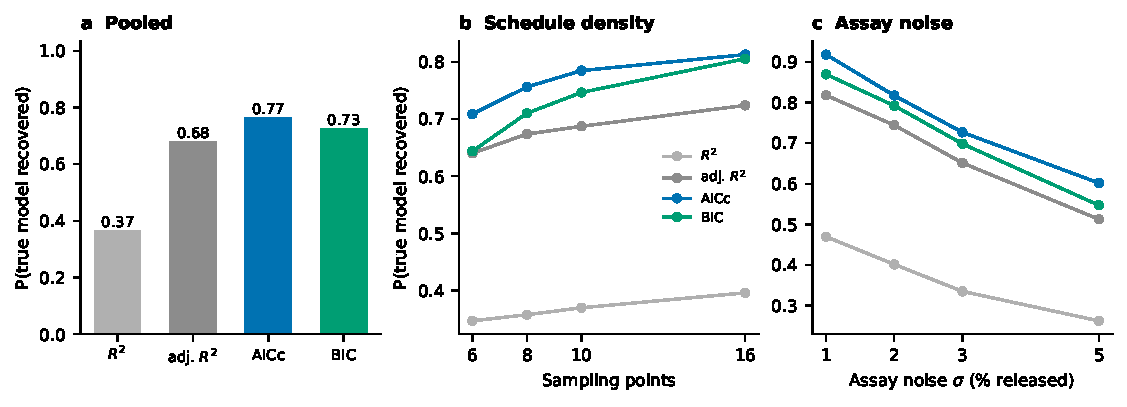
\includegraphics[width=\textwidth]{../figures/fig2_recovery.pdf}
\caption{\textbf{Recovery of the generating model by selection rule.}
(a) Pooled over all conditions. (b, c) Broken down by schedule density and
assay noise. Denser sampling and lower noise help every rule, but do not
close the gap between $R^2$ and the information criteria.}
\label{fig:recovery}
\end{figure}

\begin{figure}[t]
\centering
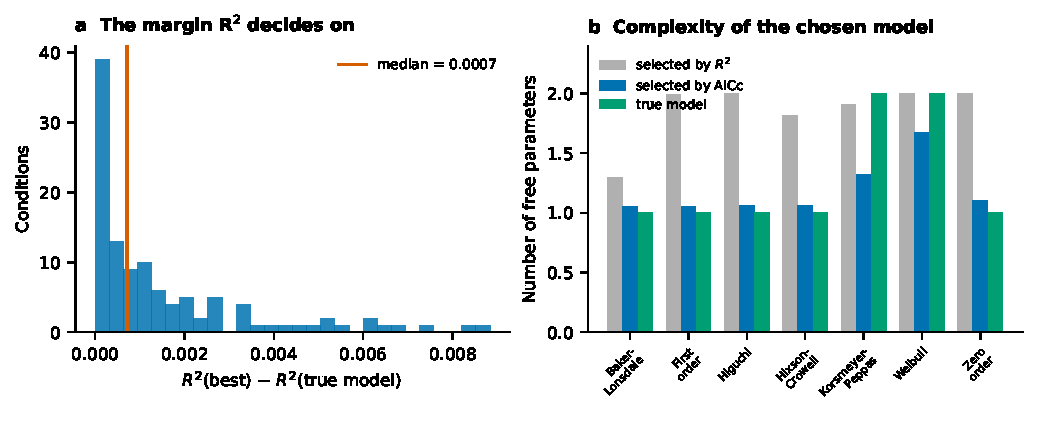
\includegraphics[width=\textwidth]{../figures/fig3_r2_gap.pdf}
\caption{\textbf{What $R^2$ is actually deciding on.} (a) Distribution across
conditions of the $R^2$ margin between the panel best and the true model.
(b) Mean number of free parameters in the selected model, against the truth.}
\label{fig:gap}
\end{figure}

\subsection{Where each rule fails}

Table~\ref{tab:selection} breaks recovery down by generating model, and the
pattern of errors is more informative than the rates. On Higuchi data $R^2$
named \HigPickRtwo{} in \HigPickRtwoF{} of profiles; on first order data it
named \FoPickRtwo{} in \FoPickRtwoF{}. These are not random errors, they are
the two most frequently reported conclusions in the applied dissolution
literature, and this study generates both of them from data containing
neither.

AICc is not uniformly better, and the case where it is worse is worth stating
plainly. On Korsmeyer-Peppas data with $n=0.42$, AICc recovered the truth
only \KPRecAICc{} of the time, naming \KPPickAICc{} instead in
\KPPickAICcF{}; $R^2$ scored \KPRecRtwo{} here. A one-parameter model
approximates a power law with $n$ near the diffusion exponent closely enough
that parsimony correctly refuses to pay for the second parameter. That is the
intended behaviour of an information criterion rather than a defect, but it
means AICc should be read as identifying the simplest model the data support,
not as identifying physical truth.

% generated by examples/make_report_numbers.py
\begin{table}[t]
\centering
\small
\caption{Percentage of profiles in which each rule recovered the generating model, by truth. $k$ is the number of free parameters in the true model. Pooled over schedules and noise levels, 400 replicates per condition.}
\label{tab:selection}
\begin{tabular}{lcrrrr}
\toprule
Generating model & $k$ & $R^2$ & adj. $R^2$ & AICc & BIC \\
\midrule
Baker-Lonsdale & 1 & 70.2 & 80.3 & 94.5 & 84.7 \\
First order & 1 & 0.0 & 65.7 & 86.7 & 74.4 \\
Higuchi & 1 & 0.0 & 64.7 & 89.2 & 74.5 \\
Hixson-Crowell & 1 & 18.3 & 63.6 & 86.0 & 71.5 \\
Korsmeyer-Peppas & 2 & 80.2 & 65.1 & 30.8 & 56.6 \\
Weibull & 2 & 88.5 & 82.3 & 61.9 & 79.5 \\
Zero order & 1 & 0.0 & 55.2 & 86.9 & 67.3 \\
\bottomrule
\end{tabular}
\end{table}


Conditions helped all rules in the same direction and by similar amounts:
AICc recovery rose from \RecAICcSix{} at six points to \RecAICcSixteen{} at
sixteen, and from \RecAICcHighNoise{} at $\sigma=5$ to \RecAICcLowNoise{} at
$\sigma=1$. No achievable sampling density rescues $R^2$.

\section{Experiment 2: can a mechanism be read off $n$?}

\subsection{Design}

Profiles were generated from the power law with a known exponent
$n \in \{0.35, 0.45, 0.60, 0.75, 0.95\}$, spanning the quasi-Fickian,
anomalous and super case II regions and sitting on the boundaries themselves.
Each replicate was truncated at 60\,\% released, and $n$ was then estimated
both by nonlinear least squares on $Q$ and by the log-log linear regression
used in most published analyses. A residual bootstrap \cite{efron1979,davison1997} of \mechNboot{}
resamples gave an interval for the nonlinear estimate.
\mechNcond{} conditions, \mechNrep{} replicates each.

\subsection{What limits a mechanistic assignment}

The truncation rule bites harder than the schedule suggests, and this was the
first thing that surprised me. Twelve scheduled
points leave \KeptTwelve{} below the cutoff on average and six leave
\KeptSix{}, so a schedule that looks twice as dense yields roughly twice as
many usable points but all of them crowded into the early part of the curve,
where the power law is flattest and $n$ is least well determined.

The mean 95\,\% bootstrap interval for $n$ was \CIWidth{} wide, against an
anomalous band of $0.44$ (Figure~\ref{fig:mech}b). That is the first surprise: on average the interval
is comfortably narrower than the class it has to fit inside, so the blanket
claim that $n$ is never precise enough to support a mechanism is not what the
data say. Nevertheless the interval lay entirely inside one mechanistic class
in only \SingleClass{} of profiles.

The two facts are reconciled by where the true exponent sits
(Figure~\ref{fig:mech}c). Splitting the conditions by distance from a
Ritger-Peppas boundary separates them almost completely
(Table~\ref{tab:mech}). For true exponents at least $0.10$ from a
boundary ($n=\InteriorNs$) the point estimate landed in the correct class
\ClassCorrectInterior{} of the time and the interval fitted inside one class
in \SingleClassInterior{}. For exponents on or within $0.06$ of a boundary
($n=\BoundaryNs$) the same numbers fall to \ClassCorrectBoundary{} and
\SingleClassBoundary{}. At $n=0.45$, which is the slab boundary itself, the
classification is a coin toss, as it must be.

This is a more useful conclusion than a blanket one, and it is not the one I
expected. A mechanism read off $n$ is reliable when $n$ falls well inside a
class, and close to worthless when it falls near a boundary. The catch is that
the analyst cannot tell which situation applies from the point estimate alone,
because a value of $0.47$ looks exactly as authoritative as a value of $0.60$.
Computing the interval is what separates them, and it costs seconds.

\begin{figure}[t]
\centering
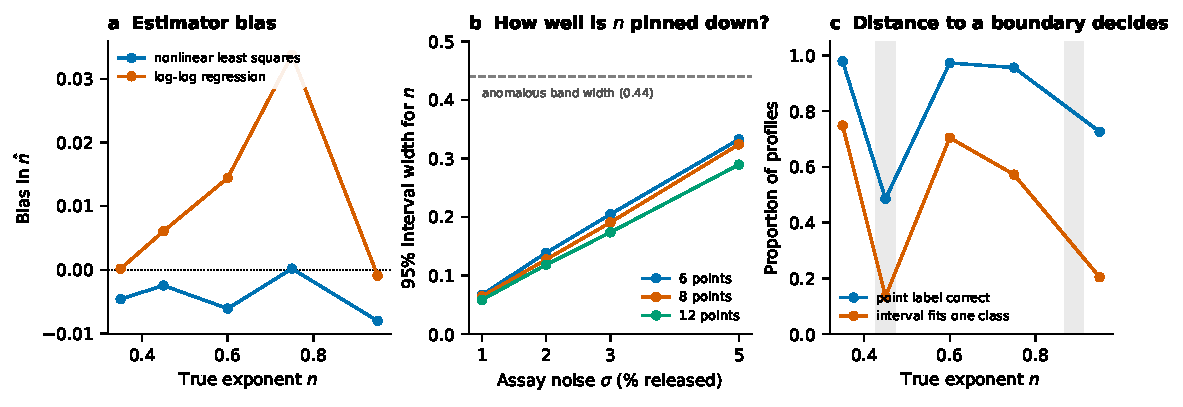
\includegraphics[width=\textwidth]{../figures/fig4_mechanism.pdf}
\caption{\textbf{Estimating the Peppas exponent under the 60\,\% rule.}
(a) Bias of the two estimators against the true exponent. (b) Width of the
95\,\% bootstrap interval for $n$; the dashed line is the width of the whole
anomalous transport band, so on average the interval is narrower than the
class it must fit inside. (c) Reliability against the true exponent, with the
Ritger-Peppas boundaries shaded: what decides whether a mechanism can be
assigned is not precision in general but distance from a boundary.}
\label{fig:mech}
\end{figure}

\subsection{The intervals are narrower than they should be}

Bootstrap coverage of the true $n$ was \Coverage{} against a nominal
95\,\%. The shortfall tracked the number of points (\CovSix{} on a six
point schedule, \CovEight{} on eight, \CovTwelve{} on twelve) and was
essentially flat in $\sigma$. That pattern points at degrees of freedom
rather than at noise. Fitted residuals are shrunk relative to
the true errors because the fit has already absorbed $k$ of the $n$ degrees of
freedom, and with four to six usable points and two parameters that is a large
fraction of them.

A dedicated calibration experiment confirms the diagnosis. At $n=\calNtrue$ and $\sigma=\calSigma$,
with \calNrep{} replicates and \calNboot{} resamples, the plain residual
bootstrap covered the truth \CovPlain{} of the time and produced intervals
\RatioPlain{} times the width of the estimator's actual sampling
distribution. Rescaling the residuals by $\sqrt{n/(n-k)}$ before resampling
raised coverage to \CovResc{} at a width ratio of \RatioResc{}, with the
largest gain on the sparsest schedule (\CovPlainSix{} to \CovRescSix{} at six
points). The package applies the rescaling by default; Experiment 2 was run
without it, so the interval widths and single-class proportions reported above
are optimistic, and the true rate at which a profile supports a single
mechanistic label is lower than \SingleClass{}.

I could have switched the correction on before running anything and reported
only the corrected numbers. Reporting both seemed more honest, and more
useful: an interval that undercovers is worse than no interval at all,
because it still carries the authority of a number.

\subsection{The linearisation is not free}

Taking logs of both sides of $Q=k_{KP}t^{\,n}$ and regressing $\ln Q$ on
$\ln t$ is convenient and nearly universal. It is not equivalent to fitting
the model to the data, because the transform reweights the points: if the
assay error is roughly constant in percent released, the early low points,
where the relative error is largest, are given the most leverage. Averaged over all conditions the bias was
modest for both, \BiasLog{} for the linearisation against \BiasNLS{} for
nonlinear least squares; the cost shows up in the spread rather than the
centre. Root mean square error was \RmseLog{} against \RmseNLS{}, so the
linearisation carries \RmseRatio{} times the error of fitting the model to the
data it was measured in. The two conventions assigned different mechanistic
labels to the same profile in \Disagreeance{} of cases, so on roughly one
profile in \DisagreeOneIn{} the reported mechanism is determined by the
fitting convention rather than by the data.

% generated by examples/make_report_numbers.py
\begin{table}[t]
\centering
\small
\caption{Estimation of the Peppas exponent by true value, pooled over schedules and noise. NLS: nonlinear least squares on percent released; LL: log-log linear regression. The last three columns are percentages of profiles. 150 replicates and 200 bootstrap resamples per condition.}
\label{tab:mech}
\begin{tabular}{ccrrrrrr}
\toprule
& & \multicolumn{2}{c}{Bias in $\hat n$} & 95\% CI & \multicolumn{1}{c}{CI in one} & \multicolumn{2}{c}{Correct class (\%)} \\
\cmidrule(lr){3-4}\cmidrule(lr){7-8}
$n$ & True class & NLS & LL & width & class (\%) & NLS & LL \\
\midrule
0.35 & Quasi-Fickian diffusion & -0.005 & +0.000 & 0.11 & 75 & 98 & 96 \\
0.45 & Anomalous & -0.002 & +0.006 & 0.13 & 14 & 49 & 51 \\
0.60 & Anomalous & -0.006 & +0.014 & 0.16 & 70 & 97 & 93 \\
0.75 & Anomalous & +0.000 & +0.034 & 0.20 & 57 & 96 & 84 \\
0.95 & Super Case II transport & -0.008 & -0.001 & 0.27 & 20 & 73 & 60 \\
\bottomrule
\end{tabular}
\end{table}


\subsection{A worked profile}

Figure~\ref{fig:worked} takes one simulated profile through the whole
pipeline: eight scheduled points, of which the 60\,\% rule keeps a subset, a
nonlinear fit, and \num{3000} bootstrap resamples of $n$ plotted against the
mechanistic boundaries. The output is not a mechanism. It is an interval, and
the honest reporting of it is the interval together with the proportion of the
resampling distribution falling in each class.

\begin{figure}[t]
\centering
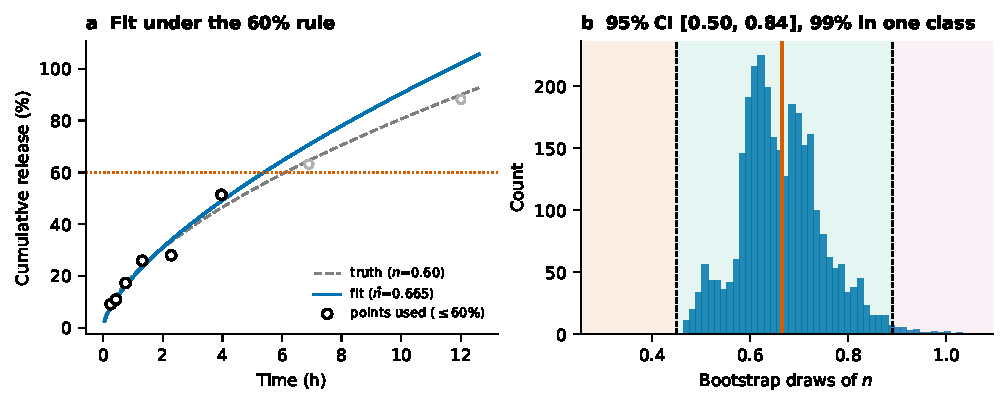
\includegraphics[width=\textwidth]{../figures/fig5_worked_example.pdf}
\caption{\textbf{One profile reported properly.} (a) The fit, with points
excluded by the 60\,\% rule shown in grey. (b) The bootstrap distribution of
$n$ against the Ritger-Peppas boundaries, shaded by mechanistic class.}
\label{fig:worked}
\end{figure}

\section{Experiment 3: is the \texorpdfstring{$f_2$}{f2} decision stable?}

The same scepticism was applied to the similarity factor
$f_2 = 50\log_{10}\!\big(100/\sqrt{1+\overline{(R-T)^2}}\big)$
\cite{moore1996}, which is computed from the means of a small number of
vessels and is compared against a fixed threshold of 50 by both the FDA and
the EMA \cite{fda1997,ema2010}. Its sampling behaviour has been examined
before \cite{shah1998}; the question here is only whether the decision it
produces is stable at the vessel counts actually used. It survives the test, which is worth saying plainly given how the rest of the
report has gone. Across \fNmc{} simulated studies
per condition, the pass or fail decision matched the truth in \fFarAcc{} of
studies whenever the true $f_2$ lay more than one unit from the threshold,
with a worst case of \fFarWorst{}; the standard deviation of the reported
$f_2$ at twelve vessels was under \fSDsmall{} units in the region that
matters. Within one unit of the threshold the decision is a coin flip, which
is unavoidable for any sharp cutoff and is not a defect of the statistic.

One real effect is worth reporting. On genuinely identical profiles $f_2$ is
biased downward, because assay noise inflates the mean squared difference:
mean $f_2$ fell to \fIdentWorst{} rather than 100 at \fIdentWorstSD{}\,\%
vessel standard deviation with \fIdentWorstN{} vessels. The bias is
conservative, in that it pushes toward declaring difference, and it is
negligible once the profiles genuinely differ (\fBiasNonIdent{} on average across all non-identical cases). A bootstrap
interval remains worth reporting near the threshold: in the worked example the
point estimate was $f_2=\fWorked{}$, nominally a pass, with a 95\,\% interval
of $[\fWorkedLo{}, \fWorkedHi{}]$ and \fWorkedP{} of resamples below 50.

\begin{figure}[t]
\centering
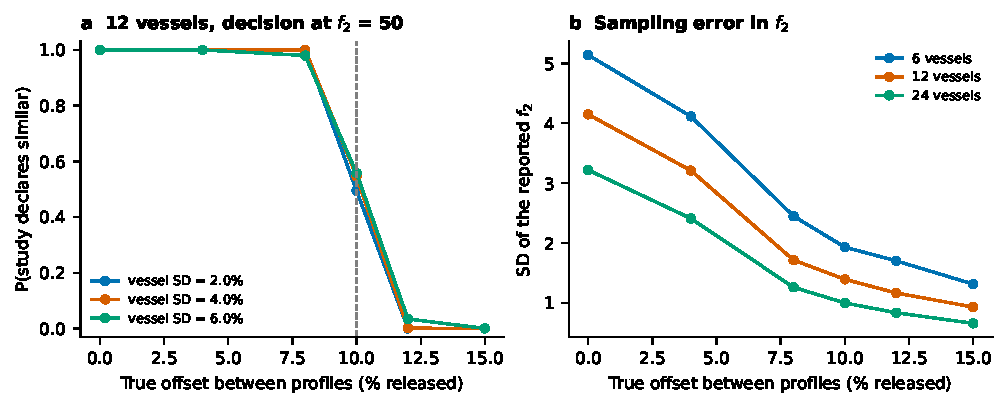
\includegraphics[width=\textwidth]{../figures/fig6_f2.pdf}
\caption{\textbf{$f_2$ is well behaved away from its threshold.}
(a) Probability that a twelve-vessel study declares similarity, against the
true offset between formulations. (b) Sampling standard deviation of the
reported $f_2$.}
\label{fig:ftwo}
\end{figure}

\section{What to report instead}

Nothing that follows is expensive, and none of it requires abandoning a model
or a workflow that already exists.

\textbf{Rank by AICc, not $R^2$, and report Akaike weights.} The computation
is three lines on top of a fit that has already been performed. Where two
models carry comparable weight, that is the result, and naming one of them a
winner discards it.

\textbf{Report $R^2$ if a journal requires it, but not as the selection
criterion,} and quote it to at least four decimals if it is quoted at all,
since the selection turns on the fourth.

\textbf{Give $n$ an interval, and rescale the residuals.} A residual
bootstrap of a few thousand resamples takes seconds, and the
$\sqrt{n/(n-k)}$ correction is one line. If the interval spans a
Ritger-Peppas boundary, the correct statement is that the data do not
distinguish the mechanisms, and that statement is more useful than a label the
data cannot support. If the interval sits well inside one class, the label is
supported and can be stated with confidence. That is the other half of the
result, and the reason to compute the interval rather than to assume the worst.

\textbf{Fit the power law to $Q$, not to $\ln Q$,} or state that the
linearisation was used and accept the bias it introduces.

\textbf{Say how many points survived the 60\,\% truncation.} Two parameters
fitted to four points is a different claim from two parameters fitted to ten,
and the distinction disappears from a paper that only reports the full
schedule.

\section{Limitations}

The study is simulation only, and deliberately so: recovery of a generating
model cannot be measured where the truth is unknown, which rules out real
profiles for this question. The consequence is that the noise model is an
assumption. Additive Gaussian error of constant variance is a reasonable
description of a UV assay over the working range, but real dissolution error
is heteroscedastic, larger at the low end and at the sampling times where
manual withdrawal dominates, and errors within a vessel are correlated across
time in a way independent draws do not reproduce. Both would widen intervals
further, so the results here are optimistic rather than pessimistic.

The candidate panel is fixed at eight models and contains one degenerate pair,
as described above. Only a slab geometry was used for the Ritger-Peppas
boundaries; a spherical device shifts them to $0.43$ and $0.85$ and narrows
the anomalous band, which would lower the single-class proportion further.
Parameter ranges were chosen to give plausible release extents, and a panel of
formulations that release only 40\,\% over the window would be a different and
probably harder problem.

The calibration experiment was run at a single exponent and noise level, so
the rescaled coverage quoted here should be read as evidence that the
diagnosis is right rather than as a general guarantee; residual rescaling is a
first order fix, and bias-corrected or accelerated intervals would be the next
step. The undercoverage also means the single-class proportions reported above
are upper bounds, which is stated where they appear but is worth repeating:
mechanism assignment near a boundary is at least as unreliable as reported,
not less.

\section{Software}

All of the above is implemented in \texttt{dissokin}, a small Python package
(\texttt{numpy}, \texttt{scipy}) providing the eight models behind one
interface, least squares fitting with AIC, AICc, BIC and Akaike weights,
residual and case bootstrap for any parameter, mechanism classification with
its resampling distribution attached, and $f_1$ and $f_2$ with a
vessel-level bootstrap. The package carries a unit test suite including
analytic checks: Baker-Lonsdale must invert its own implicit equation,
that Akaike weights sum to one, that no model releases drug backwards. Every
experiment, figure and number in this report is regenerated by the scripts in
\texttt{examples/}, and every number quoted above is inserted into this
document from the stored results rather than typed in.


\begin{thebibliography}{99}
\small
\bibitem{higuchi1961} Higuchi, T. (1961) Rate of release of medicaments from
ointment bases containing drugs in suspension. \emph{Journal of Pharmaceutical
Sciences} \textbf{50}, 874-875.
\bibitem{higuchi1963} Higuchi, T. (1963) Mechanism of sustained-action
medication: theoretical analysis of rate of release of solid drugs dispersed in
solid matrices. \emph{Journal of Pharmaceutical Sciences} \textbf{52},
1145-1149.
\bibitem{hixson1931} Hixson, A.W. and Crowell, J.H. (1931) Dependence of
reaction velocity upon surface and agitation. \emph{Industrial and Engineering
Chemistry} \textbf{23}, 923-931.
\bibitem{langenbucher1972} Langenbucher, F. (1972) Linearization of dissolution
rate curves by the Weibull distribution. \emph{Journal of Pharmacy and
Pharmacology} \textbf{24}, 979-981.
\bibitem{baker1974} Baker, R.W. and Lonsdale, H.S. (1974) Controlled release:
mechanisms and rates. In: Tanquary, A.C. and Lacey, R.E. (eds)
\emph{Controlled Release of Biologically Active Agents}, Plenum Press,
New York, 15-71.
\bibitem{hopfenberg1976} Hopfenberg, H.B. (1976) Controlled release from
eroding slabs, cylinders and spheres. \emph{ACS Symposium Series} \textbf{33},
26-32.
\bibitem{korsmeyer1983} Korsmeyer, R.W., Gurny, R., Doelker, E., Buri, P. and
Peppas, N.A. (1983) Mechanisms of solute release from porous hydrophilic
polymers. \emph{International Journal of Pharmaceutics} \textbf{15}, 25-35.
\bibitem{ritger1987a} Ritger, P.L. and Peppas, N.A. (1987) A simple equation
for description of solute release I. Fickian and non-Fickian release from
non-swellable devices in the form of slabs, spheres, cylinders or discs.
\emph{Journal of Controlled Release} \textbf{5}, 23-36.
\bibitem{ritger1987b} Ritger, P.L. and Peppas, N.A. (1987) A simple equation
for description of solute release II. Fickian and anomalous release from
swellable devices. \emph{Journal of Controlled Release} \textbf{5}, 37-42.
\bibitem{peppas1985} Peppas, N.A. (1985) Analysis of Fickian and non-Fickian
drug release from polymers. \emph{Pharmaceutica Acta Helvetiae} \textbf{60},
110-111.
\bibitem{costa2001} Costa, P. and Sousa Lobo, J.M. (2001) Modeling and
comparison of dissolution profiles. \emph{European Journal of Pharmaceutical
Sciences} \textbf{13}, 123-133.
\bibitem{zhang2010} Zhang, Y., Huo, M., Zhou, J., Zou, A., Li, W., Yao, C. and
Xie, S. (2010) DDSolver: an add-in program for modeling and comparison of drug
dissolution profiles. \emph{The AAPS Journal} \textbf{12}, 263-271.
\bibitem{moore1996} Moore, J.W. and Flanner, H.H. (1996) Mathematical
comparison of dissolution profiles. \emph{Pharmaceutical Technology}
\textbf{20}(6), 64-74.
\bibitem{shah1998} Shah, V.P., Tsong, Y., Sathe, P. and Liu, J.P. (1998)
In vitro dissolution profile comparison: statistics and analysis of the
similarity factor $f_2$. \emph{Pharmaceutical Research} \textbf{15}, 889-896.
\bibitem{fda1997} U.S. Food and Drug Administration (1997)
\emph{Guidance for Industry: Dissolution Testing of Immediate Release Solid
Oral Dosage Forms}. CDER, Rockville, MD.
\bibitem{ema2010} European Medicines Agency (2010) \emph{Guideline on the
Investigation of Bioequivalence}. CPMP/EWP/QWP/1401/98 Rev. 1, London.
\bibitem{akaike1974} Akaike, H. (1974) A new look at the statistical model
identification. \emph{IEEE Transactions on Automatic Control} \textbf{19},
716-723.
\bibitem{schwarz1978} Schwarz, G. (1978) Estimating the dimension of a model.
\emph{The Annals of Statistics} \textbf{6}, 461-464.
\bibitem{hurvich1989} Hurvich, C.M. and Tsai, C.-L. (1989) Regression and time
series model selection in small samples. \emph{Biometrika} \textbf{76},
297-307.
\bibitem{burnham2002} Burnham, K.P. and Anderson, D.R. (2002) \emph{Model
Selection and Multimodel Inference: A Practical Information-Theoretic
Approach}, 2nd edn. Springer, New York.
\bibitem{efron1979} Efron, B. (1979) Bootstrap methods: another look at the
jackknife. \emph{The Annals of Statistics} \textbf{7}, 1-26.
\bibitem{davison1997} Davison, A.C. and Hinkley, D.V. (1997) \emph{Bootstrap
Methods and their Application}. Cambridge University Press, Cambridge.
\bibitem{harris2020} Harris, C.R. et al. (2020) Array programming with NumPy.
\emph{Nature} \textbf{585}, 357-362.
\bibitem{virtanen2020} Virtanen, P. et al. (2020) SciPy 1.0: fundamental
algorithms for scientific computing in Python. \emph{Nature Methods}
\textbf{17}, 261-272.
\bibitem{hunter2007} Hunter, J.D. (2007) Matplotlib: a 2D graphics
environment. \emph{Computing in Science and Engineering} \textbf{9}, 90-95.
\end{thebibliography}

\section*{Scope}
\small
This is an independent methodological study and software project, carried out
after the author's Master's degree and unconnected to it. It is not a
peer-reviewed publication, it has not been submitted to any journal, and it
reports no experimental data. Every number reported here is produced by the
accompanying code rather than asserted, and the scripts that produce them are
in the repository.

\end{document}
